\documentclass[12pt,letterpaper]{article}

\usepackage[utf8]{inputenc}
\usepackage{color}
\usepackage{cite}
\usepackage{cancel}

%\usepackage[normalem]{ulem}
%\usepackage{epstopdf}
%\usepackage{mathbbol}
%\usepackage{hyperref}

%%%%%%%%%%%%%%%%%%%%%%%%%%%%%%
%%% PAVLOS TEMPLATE
%%%%%%%%%%%%%%%%%%%%%%%%%%%%%%
\usepackage{amsmath,amssymb,amsthm,bm}
\usepackage[usenames,dvipsnames]{xcolor}
\usepackage{graphicx}
\usepackage[T1]{fontenc}
\usepackage{pxfonts}
\usepackage{enumerate,verbatim,cite}
\usepackage[margin=1in]{geometry}
\usepackage{fancyhdr}


\pagestyle{fancy}
\addtolength{\footskip}{\baselineskip}
\renewcommand{\headrulewidth}{0pt}
\renewcommand{\footrulewidth}{0.4pt}
\fancyhf{}
\fancyfoot[L]{\textit{Last Modified: \today}}
\fancyfoot[C]{\thepage}
\usepackage[pdftex,bookmarks,hyperfigures,colorlinks
						,urlcolor=blue
						,citecolor=blue
						,linkcolor=blue
						,pdfstartview=FitH]{hyperref}


\renewcommand{\r}{{\bf r}}
\newcommand{\dery}{\frac{dx}{dt}}
\renewcommand{\k}{{\bf k}}
\newcommand{\be}{\begin{equation}}
\newcommand{\ee}{\end{equation}}

\newcommand{\myTitleBox}{
\noindent\makebox[\linewidth][c]{%
  %
    \parbox{\paperwidth}{%
      \hspace*{\dimexpr\hoffset+\oddsidemargin+1in\relax}%
      \begin{minipage}{\dimexpr\textwidth-2\fboxsep-2\fboxrule\relax}
      {\large\textbf{\courseTitleS}\courseTitle\hfill}\vspace{2mm}\\
%      {\large\textbf{\topicsCoveredS}\topicsCovered\hfill}\vspace{2mm}\\
      {\large\courseInstructors\hfill}\vspace{2mm}\\
%      \secAuthor\hfill\sectionTimesV\\
%      \authorContact\hfill\sectionTime\\
      \end{minipage}
    %
  }%
}
}


\date{}
%%%%%%%%%%%%%%%%%%%%%%%%%%%%%
%%%%%% END PAVLOS CODE
%%%%%%%%%%%%%%%%%%%%%%%%%%%%%


% bold vectors
\newcommand{\xx}{{\bf x}}
\newcommand{\yy}{{\bf y}}
\newcommand{\X}{\mathbf{X}}
\newcommand{\bmu}{{\bm{\mu}}}
\newcommand{\bbeta}{{\bm{\beta}}}
\newcommand{\etab}{{\bm{\eta}}}

% 
\newcommand{\yi}{{y_i}}
\newcommand{\mui}{{\mu_i}}
\newcommand{\thi}{{\theta_i}}
\newcommand{\phii}{{\phi_i}}
\newcommand{\ft}{{f_{\thi}}}
\newcommand{\sumi}{{\sum_{i=1}^n}}


\newcommand{\im}{\mathrm{i}}


\DeclareRobustCommand{\bbone}{\text{\usefont{U}{bbold}{m}{n}1}}

\providecommand{\pp}[1]{{\bf{\textcolor{red}{[PP:~#1]}}}}
\providecommand{\mm}[1]{{\bf{\textcolor{blue}{[MM:~#1]}}}}

\newcommand\norm[1]{\left\lVert#1\right\rVert}

\providecommand{\uu}[0]{{ \bf{u} }}
\providecommand{\yy}[0]{{ \bf{y} }}
\providecommand{\rr}[0]{{ \bf{r} }}


%\author{M. Mattheakis, G. P. Tsironis and E. Kaxiras}
%\title{Generalized Linear Models:\\Logistic Regression and Beyond  }
%\date{}
%\author{Marios Mattheakis\\CS109/??//?? Advanced Section\\
%Instructors:  M. Mattheakis, P. Protopapas \\Fall 2018, IACS, Harvard University}


\begin{document}
%\maketitle

%%
\noindent {\small{\sc{CS 209B: Advanced Topics in Data Science}  }\\
\small{\sc{Protopapas, Glickman}} \hfill \\ }

\begin{center}
\section*{Recurrent Neural Networks:\\Exploding, Vanishing Gradients \& Reservoir Computing}
\noindent {\small{\\ \small{\sc{Authors: M. Mattheakis, P. Protopapas}} }}
\end{center}
%%




\section{Exploding and Vanishing Gradient}

It seems that training a Recurrent Neural Network (RNN) is simple since we have a set of weight matrices, however, it is extremely hard. We can  analyze and understand the reason of this hardness by using the tool of  back propagation and chain rule. As we multiply all the weight matrices in forward propagation, we need to do the same in the back propagation. As we go backward the signal (derivatives) may be too strong or too weak, this is the gradient exploding or vanishing problem, respectively.  Essentially, as we go further in time the gradients become  stronger or weaker, hence for few times steps we do not observe the exploding or vanishing problem but it appears very fast as time sequence increase. Vanishing gradients make it difficult to know which direction the parameters should move to improve the loss functions, while exploding gradients make the learning unstable.
%
The forward propagation for a RNN is graphically shown in Fig. \ref {fig.RNN} reads: 
\begin{align}
\label{eq:ht}
h_t &= g_h\left( V\ x_t+ U\ h_{t-1}+b') \right), \\
\label{eq:y}
\hat y_t &= g_y\left( W\ h_t +b\right)
\end{align}
where Eq. is the hidden-to-hidden recurrence with an arbitrary activation function $g_h$ and Eq. gives the output layer with activation function $g_y$.
%
\begin{figure}[ht!]
\centering 
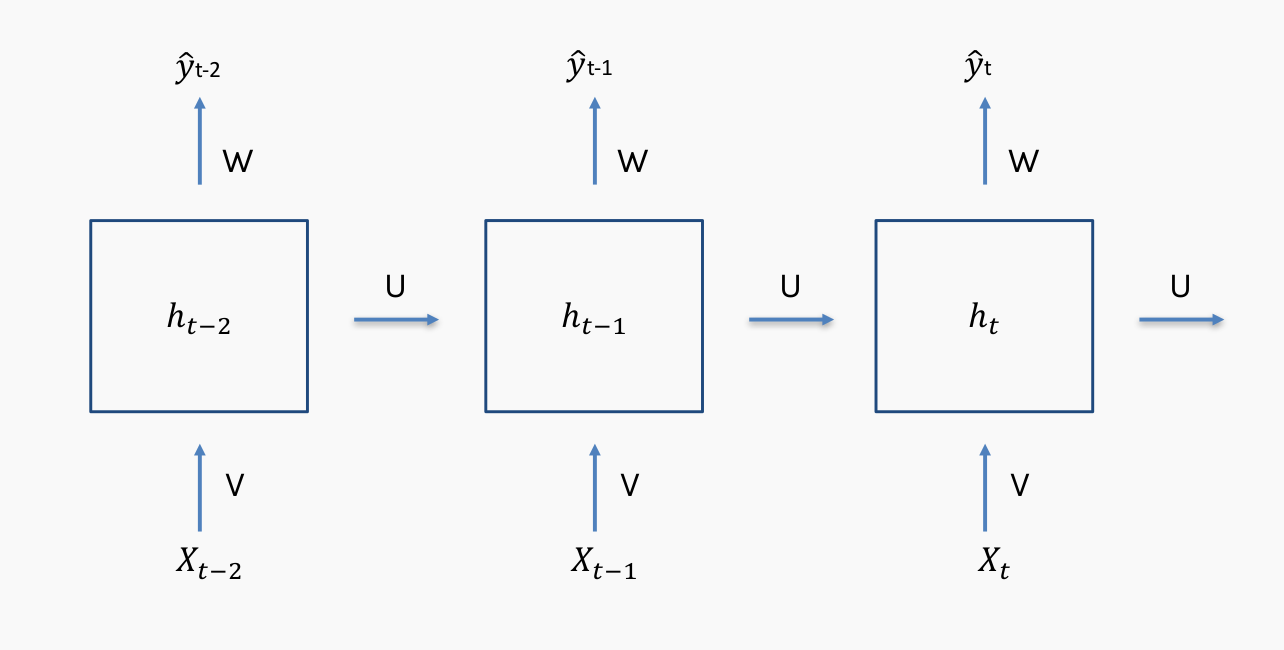
\includegraphics[scale=.2]{rnn.png}
\caption{Recurent Neural Network. \label{fig.RNN}}
\end{figure}

For the total loss  function $L$ with respect to the entire sequence in the interval $t=(1,T)$ we essentially have to sum up the loss function in all the time steps, hence
\begin{align}
\label{eq:L}
L = \sum_{t=1}^T L_t.
\end{align}
If we choose to minimize the loss function with respect to the hidden-to-hidden recurrence weights  $U$ we need to calculate the derivative 
\begin{align}
\label{eq:dL}
\frac{d L}{d U} = \sum_{t=1}^T  \frac{d L_t}{d U},
\end{align}
%
Even computing the derivative for the loss function in a single time step it requires a very large chain rule application because it essentially demands all the previous time step calculations. That becomes obvious by using the chain rule
\begin{align}
\frac{d L_t}{d U}  & = \frac{\partial L_t}{\partial \hat y_t} \frac{\partial \hat y_t}{\partial h_t}\frac{\partial h_t}{\partial U} \nonumber \\
\label{eq:dLdu}
\frac{d L_t}{d U}  & = \sum_{k=1}^t \frac{\partial L_t}{\partial \hat y_t} \frac{\partial \hat y_t}{\partial h_t}\frac{\partial h_t}{\partial h_k}\frac{\partial h_k}{\partial U}.
\end{align}
We explore deeper the Eq. (\ref{eq:dLdu}) by investigating the term ${\partial h_t}/{\partial h_k}$. To compute this term we have to use the chain rule again as:
\begin{align}
\frac{\partial h_t}{\partial h_k} &= \frac{\partial h_t}{\partial h_{t-1}}\frac{\partial h_{t-1}}{\partial h_{t-2}} \cdots \frac{\partial h_{k-1}}{\partial h_{k}} \nonumber \\
\label{eq:dhdh1}
&=\prod_{j=k+1}^t \frac{\partial h_j}{\partial h_{j-1} }.
\end{align}
The expression in the product of Eq. (\ref{eq:dhdh1}) is a derivative between two vectors and thus, it is the Jacobian matrix of the state to state transition function. Hence, the gradient ${\partial h_t}/{\partial h_k}$ is a product of Jacobian matrices each associated with a step in the forward computation. We explore further the term in the product (\ref{eq:dhdh1}) by using Eq. (\ref{eq:ht}), then we obtain
\begin{align}
\label{eq:jac}
\frac{\partial h_j}{\partial h_{j-1} } = U^T g'
\end{align}
with prime denotes derivate with respect to $h_{t-1}$. Taking the norm of the Jacobian (\ref{eq:jac}) yields
\begin{align}
\label{eq:norms}
\norm{\frac{\partial h_j}{\partial h_{j-1} }} = \norm{ U^T g'} \le \norm{U^T}\ \norm{g'} = \beta_U\ \beta_h
\end{align}
where we assumed that $\beta_U$, $\beta_h$ are the upper bound of the norms $\norm{U^T},\ \norm{g'}$, respectively. Subsequently, combining Eqs. (\ref{eq:dhdh1}) and (\ref{eq:norms}) we get
\begin{align}
\label{eq:gradientProblem}
\norm{ \frac{\partial h_t}{\partial h_k} } = \norm{ \prod_{h=k+1}^t \frac{\partial h_j}{\partial h_{j-1} } }  \le \left( \beta_U\ \beta_h \right)^{t-k} . 
\end{align}
Subsequently, as the sequence becomes larger and larger ($t\rightarrow \infty$) the term \ref{eq:gradientProblem} blows up or becomes very small whether the product  $ \beta_U\ \beta_h$ is larger or smaller that one, respectively. This is the \emph{exploding} or \emph{vanishing} gradient problem and happens very quickly since $t$ is on the exponent.

We can overpass the problem of exploding or vanishing gradients by using the \emph{clipping gradient} method, by using special RNN architectures  with leaky units such as Long-Short-Term-Memory (LSTM) and Gated Recurrent Units (GRU), or by using echo state RNNs. In the following we discuss about an echo state RNN which is called Reservoir Computing.


{\bf Exercise:} Suppose a RNN with two time steps  (2-sequence) and calculate the backprogation by using the chain rule in the derivatives. Insightful exercise.

\section{Reservoir Computing}

As it is discussed in previous section, the recurrent weights mapping from $h_{t-1}$ to $h_t$ hidden states  and the input weights mapping from $x_t$ to $h_t$ are some of the most difficult parameters to learn in an RNN. One approach to avoid this difficulty is to fix the recurrent weights such that the recurrent hidden units do a good job of capturing the history of the past inputs, and learn only the output weights. This is the backbone idea for the \emph{echo state networks} (ESN) and \emph{liquid state machines}. This networks are called \emph{reservoir computing} (RC) to denote the fact that the hidden units form a reservoir of temporal features that may capture different aspects of the history inputs (Fig. \ref{fig:rc}). An RC RNN work very well in the prediction task including forecasting the weather, controlling complex dynamical systems, pattern recognition, and predicting time series.

\begin{figure}[ht!]
\centering
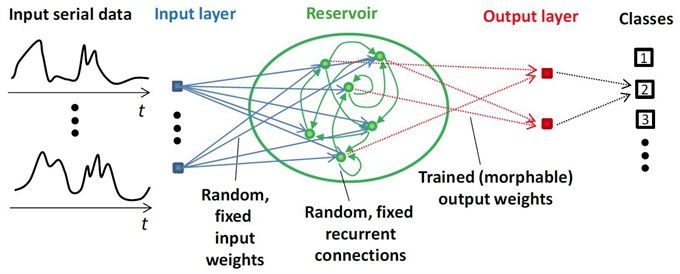
\includegraphics[scale=0.6]{rc.jpg}
\caption{Reservoir Computing Network. \label{fig:rc}}
\end{figure}

An insight way to think RC RNNs is that they map an arbitrary length sequence  (the history of the inputs up to the time $t$)  into a high-dimensional  fixed-length feature vector (the recurrent state $h_t$). Then a linear predictor, which is typically a linear regression, is applied to solve the problem of the interest. This makes RC RNNs very efficient and drastically speeds up the training since we only need to train the output weights by using the well known, from linear regression, learning algorithms. An important question that may naturally be asked is how to set the input and the recurrent weights so that a rich set of sequential history can be represented in the RNN state. The answer that is given, in the context of RC, is to view the recurrent net as a dynamical system and set the input and the recurrent weights such that the dynamical system is near the edge of stability. The stability is crucial for avoiding the exploding/vanishing gradients because it essentially means that  the eigenvalues of the state to state Jacobian are close to one and hence the gradients do not explode  or vanish (see Eq. (\ref{eq:gradientProblem})). Moreover, RC very often employs leaky hidden units that makes the hidden neurons to partially remember the its previous activation.  This type of neurons performs a leaky integration of its activation from previous time steps and thus, they are called \emph{leaky integrator neurons}. In summary, an RC is distinguished from traditional feed-forward NNs by the following qualities:
\begin{itemize}
\item The network nodes each have distinct dynamical behavior
\item Time delays of signal may occur along the network links
\item The network hidden part has recurrent connections
\item The input and internal weights are fixed and randomly chosen
\item Only the output weight are adjusted during the training.
\end{itemize}


Let us describe the formalism of an RC RNN of Fig. \ref{fig:rc}. We are seeking for a functional relationship  between $M$ given inputs $\uu (t) \in \mathrm{IR}^{M}$  and $P$ desired outputs  $\yy(t) \in \mathrm{IR}^{P}$, with $t=1,\cdots,T$ and $T$ is the number of data points in the training dataset $\{ \uu(t),\yy(t) \}_{t=1}^T$. We suppose a reservoir with $N$ dynamical and recurrent hidden nodes whose state vector is $\rr \in \mathrm{IR}^{N}$. The reservoir nodes have recurrent connections denoted by the matrix $W_\text{res}\in \mathrm{IR}^{N \times N}$.
The inputs $\uu$ are connected to the reservoir nodes through a linear input layer $W_\text{in} \in \mathrm{IR}^{M \times N}$.  In turn, the reservoir nodes are connected to the outputs through a linear output layer $W_\text{out} \in \mathrm{IR}^{N \times P}$. The hidden states and the reservoir dynamics are given by
\begin{align}
\label{eq:rcDyn}
\rr(t+\Delta t) = (1-\alpha)\rr(t) + \alpha\ f \left( W_\text{res} \rr(t) + W_\text{in} \uu(t) +{\bf b} \right)
\end{align}
where $\Delta t \ll 1$, ${\bf b}\in \mathrm{IR}^{N} $,  and $f(.)$ is the activation function usually chosen to be  sigmoid or $\tanh()$. Equation (\ref{eq:rcDyn}) describes  leaky units with $\alpha$ is the leakage rate parameter ($0<\alpha\le 1$) that controls how fast the reservoir evolves for instance, $\alpha \rightarrow 0$ the reservoir evolves slowly.  The weighted adjacent matrix $W_\text{res}$, the input matrix, and the bias vector are initially randomly drawn and then they are fixed. The output vector is taken to be a linear function of the reservoir state and defined as:
\begin{align}
\label{eq:yout}
\hat \yy(t) = W_\text{out}\rr(t) + {\bf c}
\end{align}
For the prediction task, we adjust $W_\text{out}$ and the bias vector ${\bf c}$ using a finite duration training data samples so that the resulting output represents the input data in a least-square sent. In other words, we determine the $W_\text{out}$ and ${\bf c}$  by minimizing the loss function
\begin{align}
\label{eq:loss}
\mathcal{L } = \sum_{t=1}^T || W_\text{out}\rr(t ) + {\bf c} - \hat \yy( t) ||^2 + \beta\  \text{Tr}\left( W_\text{out} W_\text{out}^T \right)
\end{align}
in the training set, where the second term is a regularization included to avoid overfitting and $\beta$ is the \emph{ridge regression parameter} which typically takes small values, and the norm $|| {\bf q} || = {\bf q}^T{\bf q}$. 
%
%Minimizing the loss function (\ref{eq:loss}) with respect  the  $W_\text{out}$ and ${\bf c}$, we obtain:
%\begin{align}
%\label{eq:wout}
%W_{out}  &= Y R\left(RR^T + \beta \mathbf{1} \right)^{-1} \\
%\label{eq:c}
%{\bf c} &= - \frac{1}{T}\sum_{t=1}^T \left( W_{out}\rr(t) - \yy(t)\right) 
%\end{align}
%where $\mathbf{1}$ is an $N\times N$ identity matrix, 
%
The great advantage of RC comparing other RNNs is that we have to estimate only the weights of the output layer, hence the training becomes very efficient and  computationally feasible for relatively large $N$.

In addition to the parameters $\alpha,\ \Delta t,\ \xi$ in Eq. (\ref{eq:rcDyn}), the reservoir dynamics depends on the parameter $D,\ \rho,$ and $\sigma$, which govern the random generation of the $W_\text{in}$ and $W_\text{res}$ as follows. The adjacency matrix $W_\text{res}$ is typically  sparse with density of non-zero matrix elements given by $D/N$, so the average degree of a reservoir node is $D$. The values of the non-zero elements are randomly drawn independently from a uniform distribution between -1 and 1. We then uniformly rescale all the elements of the $W_\text{res}$ so that the largest value of the magnitude of its eigenvalues becomes $\rho$, which is referred as the \emph{spectral radius} of the $W_\text{res}$. The elements of the $W_\text{res}$ are randomly chosen from a uniform distribution in the range $[\sigma, \ \sigma]$. There is not yet a method for optimizing these parameters, so we usually chose them in a heuristic way.

As implementation we employ an RC to predict a chaotic time-series of the Mackey-Glass system which is a standard benchmark system for time series prediction \cite{RC_paper2002}. We have one input $u(t)$, one output $\hat y(t)$ and employ $N=1000$  reservoir neurons. A 2000 step sequence is used for training the output layer and predict the time series for 1000 future step. We found that the hyper-parameters  $D/N=0.2$, $\rho=1.5$, and $\sigma=1$, are work well in the specific task. We present the results in Fig. 
\begin{figure}[ht!]
\centering
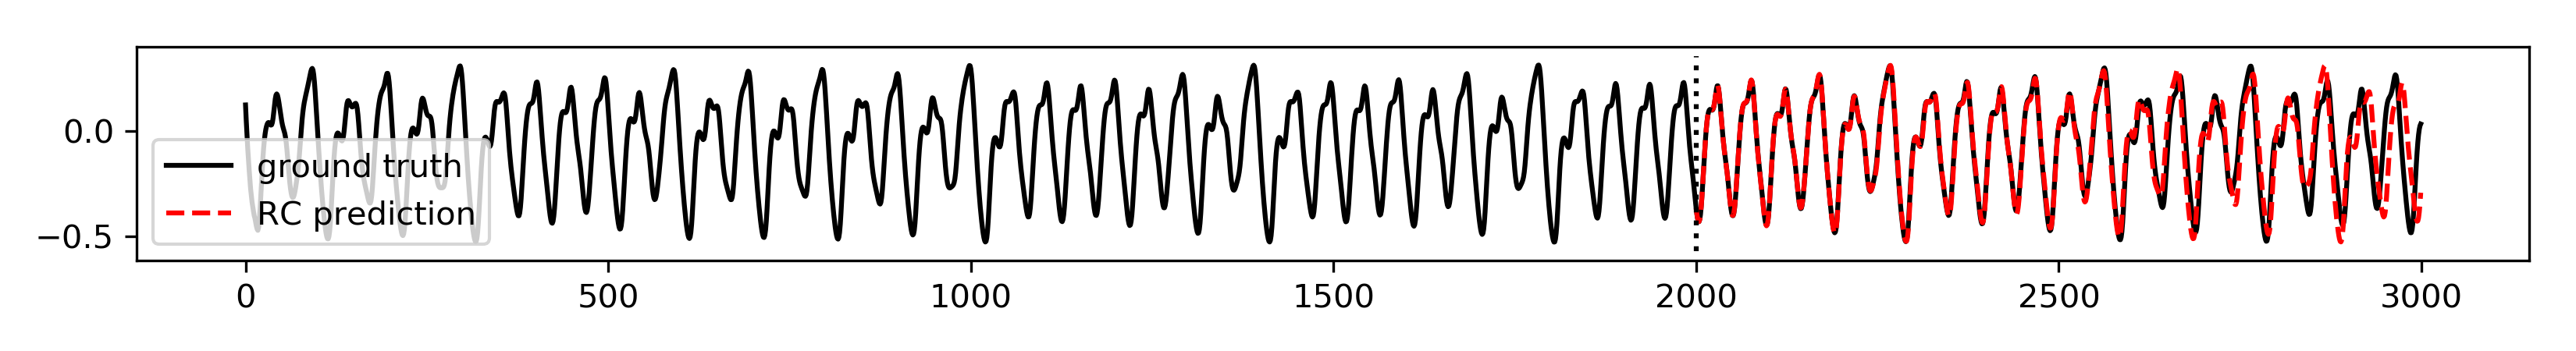
\includegraphics[scale=.5]{MG.png}
\caption{Using RC to predict the chaotic time-series of the Mackey-Glass system. Black line is the ground truth whereas red is the RC prediction. The Mean Square Error (loss function) in the prediction (in the testing set) is calculated 0.09.}
\end{figure}


\begin{thebibliography}{99}
\bibitem{goodfellow} I. Goodfellow, Y. Bengio, and A. Courville, \textit{Deep Learning}, MIT Press (2017).
%
\bibitem{RC_paper2002}  H. Jaeger, and H. Haas, \textit{Harnessing Nonlinearity: Predicting
Chaotic Systems and Saving Energy in Wireless Communication}, Science {\bf 304}, 78-80 (2014).
%
\bibitem{RC_paper2009} M. Lukosevicius, and H. Jaeger,\textit{Reservoir computing approaches to recurrent neural network training}, Computer Science Review {\bf 3} (3), 127-149 (2009).
%
\bibitem{RC_ott} Z. Lu, J. Pathak, B. Hunt, M. Girvan, R. Brockett, and E. Ott, \textit{Reservoir observers: Model-free inference of unmeasured variables in chaotic systems}, Chaos {\bf 27}, 041102 (2017).
\bibitem{RC_marios} G. N. Neofotistos, M. Mattheakis, G. Barbaris, J. Hitzanidi, G. P. Tsironis, and E. Kaxiras,  \textit{Machine learning with observers predicts complex spatiotemporal behavior}, Frontier of  Physics - Quantum Computing (forthcoming in 2019).
\end{thebibliography}

\end{document}


%%%%%%%%%%%%%%%%%%%%%%%%%%%%%%%%%%%%%%%%%%%%%%%%%%%%%%%%%%%%%%%%%%%%%%
%%%%%%%%%%%%%%%%%%%%%%%%%%%%%%%%%%%%%%%%%%%%%%%%%%%%%%%%%%%%%%%%%%%%%%
%%%%%%%%%%%%%%%%%%%%%%%%%%%%%%%%%%%%%%%%%%%%%%%%%%%%%%%%%%%%%%%%%%%%%%
%%%%%%%%%%%%%%%%%%%%%%%%%%%%%%%%%%%%%%%%%%%%%%%%%%%%%%%%%%%%%%%%%%%%%%
